\documentclass[11pt]{article}
\usepackage[a4paper,margin=26mm]{geometry}
\usepackage{amsmath,amssymb,amsthm}
\usepackage[T1]{fontenc}
\usepackage{enumitem}
\usepackage{upquote}
\usepackage{tikz}
\usepackage{xurl}
\usepackage{hyperref}
\hypersetup{colorlinks=true,linkcolor=blue,urlcolor=blue,citecolor=blue,
 pdftitle={Answers to three problems of Hak, Kozerenko and Oliynyk on the triameter of graphs},
 pdfauthor={Horace Dong}}
\newtheorem{theorem}{Theorem}
\newtheorem{lemma}[theorem]{Lemma}
\newtheorem{corollary}[theorem]{Corollary}
\newtheorem{proposition}[theorem]{Proposition}
\newtheorem*{thmA}{Theorem A}
\newtheorem*{thmB}{Theorem B}
\newtheorem*{thmC}{Theorem C}
\theoremstyle{remark}
\newtheorem{remark}[theorem]{Remark}
\DeclareMathOperator{\diam}{diam}
\DeclareMathOperator{\tr}{tr}
\DeclareMathOperator{\med}{med}
\newcommand{\FP}{\mathrm{FP}}
\newcommand{\QA}{\textup{(Q3)}}
\newcommand{\QAp}{\textup{(Q3$'$)}}
\newcommand{\QB}{\textup{(Q4)}}
\newcommand{\QBp}{\textup{(Q4$'$)}}
\setlength{\emergencystretch}{1.5em}
\DeclareUrlCommand\code{\urlstyle{tt}\def\UrlBreaks{\do\_\do\/\do\.}\def\UrlBigBreaks{}}
\newcommand{\qs}{\textquotesingle}
\newcommand{\cd}[1]{\texttt{\spaceskip=0.525em plus 0.25em minus 0.05em\relax#1}}
\tikzset{
 vx/.style={circle,fill=black,inner sep=0pt,minimum size=5pt},
 wx/.style={circle,draw,thick,fill=white,inner sep=0pt,minimum size=6.5pt},
 px/.style={rectangle,fill=black,inner sep=0pt,minimum size=5.5pt},
 pw/.style={rectangle,draw,thick,fill=white,inner sep=0pt,minimum size=6.5pt}}
\title{Answers to three problems of Hak, Kozerenko and Oliynyk\\ on the triameter of graphs}
\author{Horace Dong\\ \small Independent researcher\\
\small\texttt{maxwelldhx@gmail.com}\\
\small ORCID: \href{https://orcid.org/0009-0002-7554-7548}{0009-0002-7554-7548}}
\date{September 2026}
\begin{document}
\maketitle
\begin{abstract}
For a connected graph $G$, the triameter $\tr(G)$ is the largest value of
$d(u,v)+d(u,w)+d(v,w)$ over vertices $u,v,w$. Hak, Kozerenko and Oliynyk asked
whether every triametral triple of a median graph contains a peripheral vertex
(Problem~1), whether every diametral pair of a median graph extends to a
triametral triple (Problem~2), and whether every distance-hereditary graph has
at least one of these two properties (Problem~3). For Problem~1 we give an
$8$-vertex median counterexample, which exhaustive enumeration shows to be the
unique smallest one. Problem~2 was answered negatively on MathOverflow in
December 2025 with an $11$-vertex example; we show that the smallest
counterexample has $8$ vertices, is unique, and is also distance-hereditary.
Problem~3 has a positive answer in a stronger form: in a connected
distance-hereditary graph, every triametral triple contains a diametral pair or
every diametral pair extends to a triametral triple. The proof uses the
four-point condition of Bandelt and Mulder. The counterexamples, and the answer
to Problem~3 for graphs that satisfy the four-point condition, are formally
verified in Lean~4. The results were found by AI coding agents
working under the author's direction; their role is described at the end of
the paper.
\end{abstract}

\section{Introduction}
All graphs in this paper are finite and simple. For a connected graph $G$ with
path metric $d=d_G$, let $\diam(G)$ be its diameter, put
$d(u,v,w)=d(u,v)+d(u,w)+d(v,w)$, and let the \emph{triameter} $\tr(G)$ be the
largest value of $d(u,v,w)$ over all $u,v,w\in V(G)$~\cite{das}. A pair
$\{u,v\}$ is \emph{diametral} if $d(u,v)=\diam(G)$, a vertex is
\emph{peripheral} if it belongs to a diametral pair, and a triple $u,v,w$ is
\emph{triametral} if $d(u,v,w)=\tr(G)$. Das~\cite{das} asked whether, in a
tree, every triametral triple contains a diametral pair and every diametral
pair extends to a triametral triple. Hak, Kozerenko and Oliynyk~\cite{hko}
proved both statements for all connected block graphs~\cite[Theorem~1.2]{hko},
showed by examples that they fail for other classes, introduced weaker
versions, and posed three problems~\cite[Section~4]{hko}. In our notation, a
connected graph $G$ has property
\begin{itemize}[nosep]
\item[\QA] if every triametral triple of $G$ contains a diametral pair;
\item[\QAp] if every triametral triple of $G$ contains a peripheral vertex;
\item[\QB] if every diametral pair $\{x,y\}$ of $G$ extends to a triametral
 triple, that is, $d(x,y,z)=\tr(G)$ for some vertex $z$;
\item[\QBp] if every peripheral vertex of $G$ belongs to a triametral triple.
\end{itemize}
These are Questions~3, 3$'$, 4 and~4$'$ of~\cite{hko}. We restate the three
problems of~\cite[Section~4]{hko} in this notation.
\begin{itemize}[nosep]
\item[] \textbf{Problem 1.} Does every median graph have property \QAp?
\item[] \textbf{Problem 2.} Does every median graph have property \QB?
\item[] \textbf{Problem 3.} Does every distance-hereditary graph have property
 \QAp{} or property \QB?
\end{itemize}
Both \QAp{} and \QB{} hold for trees~\cite[Theorem~1.2]{hko} and for
hypercubes, in which every vertex is peripheral and every pair of vertices
extends to a triametral triple~\cite[Corollary~2.5]{hko}; and each of them
fails for some distance-hereditary graph~\cite[Figure~3]{hko}.

\paragraph{Results.}
Our examples for Problems~1 and~2 are the median graphs $G_1$ and $G_2$ on the vertex set $\{0,\dots,7\}$ in
Figure~\ref{fig:graphs}; the labels are those of the Lean formalisation.

\begin{thmA}
Let $G_1$ be the graph with the ten edges $01$, $02$, $04$, $06$, $13$, $23$,
$25$, $45$, $47$, $67$. Then $G_1$ is a median graph with $\diam(G_1)=4$ and
$\tr(G_1)=8$, its only peripheral vertices are $3$ and $7$, and $\{1,5,6\}$ is
a triametral triple. So $G_1$ does not have property \QAp, and the answer to
Problem~1 is negative. Moreover, every median graph with at most seven vertices
has property \QAp, and $G_1$ is, up to isomorphism, the only median graph with
eight vertices that does not.
\end{thmA}

\begin{thmB}[{a negative answer to Problem~2 was first given in~\cite{mo-a}}]
Let $G_2$ be the graph with the eight edges $02$, $03$, $06$, $12$, $25$, $34$,
$35$, $67$. Then $G_2$ is a median graph and a distance-hereditary graph with
$\diam(G_2)=4$ and $\tr(G_2)=12$, and $\{1,4,7\}$ is its only triametral triple.
So the diametral pair $\{5,7\}$ does not extend to a triametral triple, and the
peripheral vertex $5$ belongs to no triametral triple: $G_2$ has neither
property \QB{} nor property \QBp. Moreover, every median graph with at most
seven vertices has property \QB, and $G_2$ is, up to isomorphism, the only
median graph with eight vertices that does not have \QB, and also the only one
that does not have \QBp.
\end{thmB}

\begin{thmC}
Let $G$ be a connected distance-hereditary graph, and let $\{a,b,c\}$ be a
triametral triple of $G$ that contains no diametral pair. Then for every
diametral pair $\{x,y\}$ of $G$,
\[
 \max\{d(a,x,y),\,d(b,x,y),\,d(c,x,y)\}=\tr(G).
\]
Consequently every connected distance-hereditary graph has property \QA{} or
property \QB, and hence property \QAp{} or property \QB. The answer to
Problem~3 is positive.
\end{thmC}

\begin{figure}[t]
\centering
\begin{minipage}[b]{0.34\textwidth}\centering
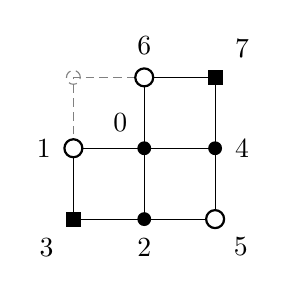
\begin{tikzpicture}[x=0.9cm,y=0.9cm,label distance=1pt]
 \draw[densely dashed,gray] (0,1)--(0,2)--(1,2);
 \node[circle,draw=gray,densely dashed,inner sep=0pt,minimum size=5pt] at (0,2) {};
 \draw (0,0)--(2,0) (0,1)--(2,1) (1,2)--(2,2) (0,0)--(0,1) (1,0)--(1,2)
  (2,0)--(2,2);
 \node[px,label=below left:{$3$}] at (0,0) {};
 \node[vx,label=below:{$2$}] at (1,0) {};
 \node[wx,label=below right:{$5$}] at (2,0) {};
 \node[wx,label=left:{$1$}] at (0,1) {};
 \node[vx,label=above left:{$0$}] at (1,1) {};
 \node[vx,label=right:{$4$}] at (2,1) {};
 \node[wx,label=above:{$6$}] at (1,2) {};
 \node[px,label=above right:{$7$}] at (2,2) {};
\end{tikzpicture}\\[3pt]
$G_1$
\end{minipage}
\qquad
\begin{minipage}[b]{0.5\textwidth}\centering
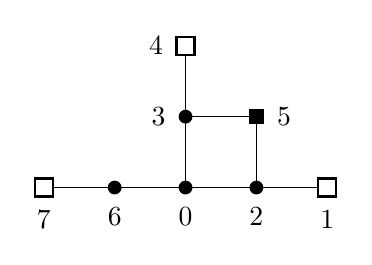
\begin{tikzpicture}[x=0.9cm,y=0.9cm,label distance=1pt]
 \draw (-2,0)--(2,0) (0,0)--(0,2) (1,0)--(1,1) (0,1)--(1,1);
 \node[pw,label=below:{$7$}] at (-2,0) {};
 \node[vx,label=below:{$6$}] at (-1,0) {};
 \node[vx,label=below:{$0$}] at (0,0) {};
 \node[vx,label=below:{$2$}] at (1,0) {};
 \node[pw,label=below:{$1$}] at (2,0) {};
 \node[vx,label=left:{$3$}] at (0,1) {};
 \node[px,label=right:{$5$}] at (1,1) {};
 \node[pw,label=left:{$4$}] at (0,2) {};
\end{tikzpicture}\\[3pt]
$G_2$
\end{minipage}
\caption{The graphs $G_1$ and $G_2$ at the grid points of
Section~\ref{sec:median}. Squares are peripheral vertices. In $G_1$ the white
vertices $1,5,6$ form a triametral triple without a peripheral vertex; in $G_2$
the white vertices $1,4,7$ form the only triametral triple.}\label{fig:graphs}
\end{figure}

The last sentences of Theorems~A and~B rest on exhaustive enumerations
(Section~\ref{sec:min}). Theorem~C holds for all finite connected graphs that
satisfy the four-point condition of Bandelt and Mulder~\cite[Theorem~2]{bm}
(Section~\ref{sec:dh}); Remark~\ref{rem:sharp} shows that it is sharp. The
counterexamples $G_1$ and $G_2$, and Theorem~C under the four-point condition,
are formally verified in Lean~4 (Section~\ref{sec:lean}).

\paragraph{Prior work.}
The negative answer to Problem~2 is not new. Hak and Kozerenko restated the
question in the Lviv Scottish Book~\cite{lsb} (volume~3, page~154, entry dated
10 February 2025), asking whether \QB, or at least \QBp, holds for median
graphs; the entry also suggests asking whether \QAp{} does, which is
Problem~1. The problem was relayed to MathOverflow as question
506431~\cite{mo-q} on 28 December 2025, and on 31 December 2025 the user
rgvalenciaalbornoz answered it~\cite{mo-a}, in an accepted answer, with an
$11$-vertex median graph made of four $4$-cycles in which both \QB{} and \QBp{}
fail. That answer does not concern \QAp. Our contribution to Problem~2 is only
the smallest counterexample of Theorem~B, and the observation that it is also
distance-hereditary.

For Problems~1 and~3 we found no earlier answer. We searched on 26 September
2026 between 06:43 and 07:21 UTC: the arXiv (its API, for triameter,
triametral, triametric and for the papers of Kozerenko); the works
citing~\cite{hko} listed by OpenAlex and Semantic Scholar, read in full where
accessible; Crossref; zbMATH Open; MathDB; MathOverflow and Mathematics Stack
Exchange, through the Stack Exchange API; the Lviv Scottish Book; Wikipedia;
MathWorld; GitHub (code, commits, issues, pull requests, repositories); the
repositories \texttt{trureturing}~\cite{tru},
\texttt{formal-conjectures}~\cite{fc} and \texttt{SCOPE2026}~\cite{scope} of
AI-assisted work on open problems; A.~Hak's bachelor thesis (2022); and web
search. The Wikipedia article on the triameter~\cite{wiki}, last
revised on 19 October 2025, before the MathOverflow answer, lists Problem~2 as
open and suggests studying \QAp{} and \QBp{} for median graphs; the
paper~\cite{koz} (29 August 2026) mentions such questions for median and
distance-hereditary graphs without answering them.\footnote{A figure caption in~\cite{wiki} calls the graph $G$
of~\cite[Figure~3]{hko} ($K_{2,3}$ with a pendant vertex) a median graph. It
lacks \QAp, but it is not median, as its vertices $a,b,c$ have two medians; so
it does not answer Problem~1.} Some searches
failed: the keyword searches of OpenAlex and Semantic Scholar returned HTTP
error~429 (rate limit), and we used keyword searches of Crossref instead; one
citing paper, in \emph{Symmetry}, was judged from its abstract, as its full
text was not accessible to us; and a citation search in zbMATH Open gave no
usable result. We did not search Google Scholar, Scopus, Web of Science
or ResearchGate. General web search did not find the MathOverflow thread, which
we found only through the Stack Exchange API. A final check on 26 September
2026 between 15:49 and 15:52 UTC (the arXiv, GitHub, MathDB and MathOverflow)
found nothing new. This reports the coverage of our searches, not a guarantee
of priority.

We quote~\cite{hko} from its arXiv version~1; its theorem, figure and problem
numbers refer to that version.

\section{Definitions and readings}\label{sec:defs}
Let $G$ be a connected graph with path metric $d$ and $D=\diam(G)$. A vertex
$u$ is peripheral if and only if its eccentricity $\max_vd(u,v)$ equals $D$. As
in~\cite{hko}, the vertices in the definition of $\tr(G)$ need not be distinct.
For a diametral pair $\{x,y\}$ and any vertex $z$, the triangle inequality gives
$d(x,y,z)\ge2d(x,y)=2D$; hence $2D\le\tr(G)\le3D$~\cite[Proposition~2.1]{hko}.
For vertices $u,v$ let $[u,v]=\{x:d(u,x)+d(x,v)=d(u,v)\}$. A connected graph is
a \emph{median graph} if $|[u,v]\cap[u,w]\cap[v,w]|=1$ for all vertices
$u,v,w$~\cite{mulder}; the unique vertex is the \emph{median} of $u,v,w$. A
connected graph is \emph{distance-hereditary} if every connected induced
subgraph $H$ is isometric, that is, $d_H(u,v)=d_G(u,v)$ for all
$u,v\in V(H)$~\cite{howorka}.

\paragraph{Readings.}
A triple with a repeated vertex has $d(u,u,v)=2d(u,v)\le2D\le\tr(G)$, with
equality only if $\tr(G)=2D$ and $\{u,v\}$ is diametral; so allowing repeated
vertices changes nothing in \QA{} and \QAp. In \QB, the vertex $z$ may be
required to differ from $x$ and $y$ (the \emph{strong reading}) or not (the
\emph{weak reading}). If $G$ has at least three vertices the readings agree: if
some $z\in\{x,y\}$ works, then $\tr(G)=2D$, and then every $z$ works; similarly
for \QBp. Our counterexamples refute every reading, and Theorem~C holds under
the strong one. Also, \QB{} implies \QBp, since a peripheral vertex $x$ lies in
a diametral pair, which extends to a triametral triple containing $x$.

The sentence of~\cite{hko} that introduces Problem~2 describes \QA, while
the problem names Question~4. As~\cite[Figure~4]{hko} already shows that \QA{}
fails for median graphs, and the restatement~\cite{lsb,mo-q} concerns \QB, we
read Problem~2 as stated ($G_1$ also lacks \QA). Problem~3 could be read for
the class (all distance-hereditary graphs have \QAp, or all have \QB), but the
two graphs of~\cite[Figure~3]{hko}, shown just before the problem, refute this
reading; so we read it for each graph. As both vertices of a diametral pair are
peripheral, \QA{} implies \QAp; so Theorem~C gives more than a positive answer,
and it also gives \QAp{} or \QBp.

\section{Two median graphs}\label{sec:median}
We prove Theorems~A and~B, except for their last sentences, by placing $G_1$
and $G_2$ in the integer grid. For $u,v\in\mathbb Z^k$ let
$\|u-v\|=\sum_i|u_i-v_i|$, and for integers $a,b,c$ let $\med(a,b,c)$ be the
middle one of the three. For $S\subseteq\mathbb Z^k$ let $\Gamma(S)$ be the
graph on $S$ in which $u$ and $v$ are adjacent when $\|u-v\|=1$.

\begin{lemma}\label{lem:grid}
Let $S\subseteq\mathbb Z^k$ be finite, and suppose that
\textup{(a)} $d_{\Gamma(S)}(u,v)=\|u-v\|$ for all $u,v\in S$, and
\textup{(b)} $S$ is closed under coordinatewise medians: for $u,v,w\in S$, the
point $m(u,v,w)$ with coordinates $\med(u_i,v_i,w_i)$ lies in $S$. Then
$\Gamma(S)$ is a median graph, the median of $u,v,w$ is $m(u,v,w)$, and
\begin{equation}\label{eq:tri}
 d(u,v,w)=2\sum_{i=1}^k\bigl(\max\{u_i,v_i,w_i\}-\min\{u_i,v_i,w_i\}\bigr)
 \qquad\text{for all }u,v,w\in S.
\end{equation}
\end{lemma}
\begin{proof}
By (a), $\Gamma(S)$ is connected. For integers $a,b,z$ we have
$|a-z|+|z-b|\ge|a-b|$, with equality if and only if $z$ lies between $a$
and~$b$. Summing over the coordinates and using (a), a point $z\in S$ lies in
$[u,v]$ if and only if $z_i$ lies between $u_i$ and $v_i$ for every $i$. An
integer lies between each two of $a,b,c$ if and only if it equals
$\med(a,b,c)$: if $a\le b\le c$, it must lie between $a$ and $b$ and between
$b$ and $c$, so it equals $b$, and $b$ does lie between each two. Hence
$[u,v]\cap[u,w]\cap[v,w]=\{m(u,v,w)\}\cap S=\{m(u,v,w)\}$ by~(b). Finally, if
$a\le b\le c$ then $|a-b|+|a-c|+|b-c|=2(c-a)$; applying this in each
coordinate and using (a) gives~\eqref{eq:tri}.
\end{proof}

Condition~(a) holds if any two points $u,v\in S$ are joined by a
\emph{monotone lattice path} in $S$, that is, a path in $\Gamma(S)$ along which
every coordinate changes monotonically. Such a path has length $\|u-v\|$, and
no path is shorter, since along each edge the value of $\|x-v\|$ changes by
one.

\begin{proof}[Proof of Theorem~A, except the last sentence]
Place the vertices of $G_1$ at the points
\[
 3=(0,0),\ 2=(1,0),\ 5=(2,0),\ 1=(0,1),\ 0=(1,1),\ 4=(2,1),\ 6=(1,2),\ 7=(2,2)
\]
(Figure~\ref{fig:graphs}). These are the points of
$S_1=\{0,1,2\}^2\setminus\{(0,2)\}$, and the pairs of them at distance~$1$ are
exactly the ten edges of $G_1$; so $G_1=\Gamma(S_1)$. Two points of $S_1$ are
joined by a monotone lattice path in $\{0,1,2\}^2$. If it passes through the
corner $(0,2)$, it does so between the grid neighbours $(0,1)$ and $(1,2)$ of
the corner, and replacing $(0,2)$ by $(1,1)$ gives a monotone lattice path in
$S_1$. So (a) holds. For (b), suppose that $m(u,v,w)=(0,2)$ for some
$u,v,w\in S_1$. Then two of $u,v,w$ have first coordinate $0$ and two have
second coordinate $2$; one of them has both, and so equals $(0,2)\notin S_1$, a
contradiction. By Lemma~\ref{lem:grid}, $G_1$ is a median graph.

The distance $\|u-v\|$ between points of $S_1$ is at most $4$, with equality
only for $\{u,v\}=\{(0,0),(2,2)\}$, as $(0,2)\notin S_1$. Hence
$\diam(G_1)=4$, the only diametral pair is $\{3,7\}$, and the peripheral
vertices are $3$ and $7$. By~\eqref{eq:tri}, $d(u,v,w)\le2(2+2)=8$, and the
vertices $1=(0,1)$, $5=(2,0)$ and $6=(1,2)$ attain this bound, since in each
coordinate their values range from $0$ to $2$. So $\tr(G_1)=8$, and
$\{1,5,6\}$ is a triametral triple that contains neither $3$ nor $7$. Its
distances are $d(1,5)=3$, $d(1,6)=2$ and $d(5,6)=3$, so it contains no
diametral pair either. (On the other hand, $G_1$ has \QB, as
$\tr(G_1)=2\diam(G_1)$.)
\end{proof}

\begin{proof}[Proof of Theorem~B, except the last sentence]
Place the vertices of $G_2$ at the points
\[
 7=(-2,0),\ 6=(-1,0),\ 0=(0,0),\ 2=(1,0),\ 1=(2,0),\ 3=(0,1),\ 5=(1,1),\ 4=(0,2).
\]
The pairs of these points at distance~$1$ are exactly the eight edges of
$G_2$, so $G_2=\Gamma(S_2)$, where $S_2$ consists of the row
$R=\{(t,0):-2\le t\le2\}$ and the points $(0,1)$, $(1,1)$ and $(0,2)$. Two
points of $R$ are joined along $R$; a point $(t,0)$ is joined to $(0,1)$ and to
$(0,2)$ by going along $R$ to $(0,0)$ and then up, and to $(1,1)$ by going
along $R$ to $(1,0)$ and then up; and $(1,1),(0,1),(0,2)$ is a monotone path.
So (a) holds. For (b), let $u,v,w\in S_2$ and $m=m(u,v,w)$. If at most one of
$u,v,w$ lies outside $R$, then $m_2=0$ and $m\in R$. Otherwise two of them lie
in $\{(0,1),(1,1),(0,2)\}$, so that $m_1\in\{0,1\}$ and $m_2\in\{1,2\}$. If
$m_2=1$, then $m\in S_2$; if $m_2=2$, then two of $u,v,w$ equal $(0,2)$, and
$m=(0,2)$. By Lemma~\ref{lem:grid}, $G_2$ is a median graph.

The first coordinates of the points of $S_2$ range over $[-2,2]$ and the
second over $[0,2]$. So by~\eqref{eq:tri}, $d(u,v,w)\le2(4+2)=12$, with
equality if and only if the triple contains the only point with first
coordinate $-2$ (vertex $7$), the only point with first coordinate $2$
(vertex~$1$) and the only point with second coordinate $2$ (vertex $4$). Hence
$\tr(G_2)=12$, and every triametral triple consists of $1,4,7$, which are
pairwise at distance $4$. One checks from the coordinates that no two vertices
are at distance more than $4$; so $\diam(G_2)=4$, and
$d(5,7)=\|(1,1)-(-2,0)\|=4$ shows that $\{5,7\}$ is a diametral pair and $5$ is
peripheral. As $5\notin\{1,4,7\}$, no triple containing $5$ is triametral. So
$d(5,7,z)<12$ for every vertex $z$, and $G_2$ has neither \QB{} nor \QBp. It has \QA, since its only triametral triple
consists of diametral pairs.

Finally, $G_2$ is distance-hereditary. It is obtained from the edge $02$ by
attaching a pendant vertex $5$ at $2$, then adding a vertex $3$ adjacent to the
two neighbours $0$ and $5$ of $2$ (a false twin of $2$), and then attaching
pendant vertices $1$ at $2$, $4$ at $3$, $6$ at $0$ and $7$ at $6$. Attaching a
pendant vertex and adding a twin preserve distance-heredity; this is the easy
direction of~\cite[Theorem~1]{bm}.
\end{proof}

So \QB{} fails even for graphs that are both median and distance-hereditary;
by Theorem~C, this can happen only in graphs with property \QA, like $G_2$. The
example of~\cite{mo-a} is not distance-hereditary: in its notation, the
vertices $b,v_2,s,w_1,x$ induce a path of length~$4$, while $d(b,x)=2$.

\section{The smallest counterexamples}\label{sec:min}
The last sentences of Theorems~A and~B were proved by two independent
exhaustive enumerations of the median graphs with at most eight vertices. The
programs and their logs are in version~1.4.0 of the repository~\cite{repo},
directory \texttt{certificates/hko-triameter/}.

The first enumeration, a C program, runs for each $n\le8$ over all
$2^{n(n-1)/2}$ graphs on $\{0,\dots,n-1\}$, keeps the connected ones, tests the
median property from the definition for all triples, and for each median graph
tests \QA, \QAp{} and \QB, the last under both readings. Isomorphism classes
come from canonical forms, over all $n!$ relabellings for $n\le7$ and over
relabellings refined by vertex invariants for $n\le8$; the two agree for
$n\le7$. The numbers of
connected labelled graphs, $1,1,4,38,728,26704,1866256,251548592$ for
$n=1,\dots,8$, are those of sequence A001187 of the OEIS~\cite{oeis}, and the
numbers of median graphs up to isomorphism, $1,1,1,3,4,11,23,69$, are those of
sequence A292623 (median graphs on $n$ nodes). No median graph with at most
seven vertices lacks \QAp{} or \QB. Of the $1{,}008{,}904$ labelled median
graphs with eight vertices, exactly $20{,}160$ lack \QAp{} and exactly
$20{,}160$ lack \QB. A check over all $8!$ bijections shows that these are the
labelled copies of $G_1$ and of $G_2$, respectively; each of $G_1$ and $G_2$
has exactly two automorphisms, and $8!/2=20{,}160$.

The second enumeration, a Python program, takes all graphs with at most seven
vertices from the graph atlas of the NetworkX library and tests the median
property from the definition, with Floyd--Warshall distances. For $n=8$ it
uses two facts: a median graph has no triangle, since for a triangle $u,v,w$
the intervals $\{u,v\}$, $\{u,w\}$, $\{v,w\}$ have no common vertex; and every
connected graph has a vertex whose removal leaves it connected, such as a leaf
of a spanning tree. So every median graph with eight vertices arises from one
of the $59$ connected triangle-free graphs with seven vertices by adding a
vertex adjacent to a nonempty independent set. The program forms all $1{,}857$
such graphs and reduces the median ones up to isomorphism with NetworkX. It
finds the same numbers of median graphs, no violation for $n\le7$, and for
$n=8$ exactly one median graph lacking \QAp{} and one lacking \QB, isomorphic
to $G_1$ and $G_2$. Finally, as \QB{} implies \QBp, no median graph with at most
seven vertices lacks \QBp, and $G_2$ is the only one with eight vertices that
does.

\section{Distance-hereditary graphs: proof of Theorem C}\label{sec:dh}
Bandelt and Mulder~\cite[Theorem~2]{bm} proved that, for a connected
graph~$G$, the following conditions, among others, are equivalent (we keep
their numbering). (i)~$G$ is distance-hereditary. (vii)~For any four vertices
$u,v,w,x$, at least two of the three distance sums $d(u,v)+d(w,x)$,
$d(u,w)+d(v,x)$ and $d(u,x)+d(v,w)$ are equal. (viii)~$G$ satisfies (vii),
and if the two smaller of these sums are equal, then the largest one exceeds
them by at most~$2$. The
characterisation quoted in~\cite[Section~3.2]{hko} is (i)$\Leftrightarrow$(vii);
we need (viii). For integers $A,B,C$ write $\FP(A,B,C)$ if two of them are equal
and the third is at most their common value plus~$2$. This is symmetric in
$A,B,C$, and three sums satisfy it exactly when they satisfy the requirements of
(viii): if the two larger sums are equal, the third is at most their value, and if the two
smaller ones are equal, (viii) bounds the largest. A connected graph $G$ satisfies the \emph{four-point condition} if
$\FP\bigl(d(u,v)+d(w,x),\,d(u,w)+d(v,x),\,d(u,x)+d(v,w)\bigr)$ holds for all
$u,v,w,x\in V(G)$. By the implication (i)$\Rightarrow$(viii) of~\cite[Theorem~2]{bm}, every
connected distance-hereditary graph satisfies the four-point condition. This is
the only fact about distance-hereditary graphs that we use.

The core of the proof is a statement about integers, in which $a,b,c$ are
three labels.

\begin{lemma}\label{lem:core}
Let $D$, $e_{ab},e_{ac},e_{bc}$, $p_a,p_b,p_c$ and $q_a,q_b,q_c$ be integers,
put $e_{vu}=e_{uv}$ and $T=e_{ab}+e_{ac}+e_{bc}$, and suppose that for all distinct
$u,v\in\{a,b,c\}$
\[
 \text{(E)}\ \ e_{uv}\le D-1,\qquad
 \text{(F)}\ \ \FP(D+e_{uv},\,p_u+q_v,\,p_v+q_u),\qquad
 \text{(N)}\ \ D+p_u+q_u\le T-1.
\]
These conditions are inconsistent.
\end{lemma}
\begin{proof}
Put $s_u=p_u+q_u$ and $t_u=p_u-q_u$. Fix distinct $u,v\in\{a,b,c\}$, and let
$w$ be the third label. By (F), at least one of the following holds:
\begin{align*}
 &(\mathrm A_{uv})\quad D+e_{uv}=p_u+q_v;\qquad
 (\mathrm A_{vu})\quad D+e_{uv}=p_v+q_u;\\
 &(\mathrm C_{uv})\quad p_u+q_v=p_v+q_u\ \text{ and }\ D+e_{uv}\le p_u+q_v+2.
\end{align*}

\emph{Claim 1. If $(\mathrm A_{uv})$ holds, then
$q_v-q_u\ge2D+1-e_{uw}-e_{vw}$ and $t_u-t_v\ge6$.} Put
$k=2D+1-e_{uw}-e_{vw}$; by (E), $k\ge3$. Substituting $p_u=D+e_{uv}-q_v$ into
(N) for $u$ gives $2D+e_{uv}-q_v+q_u\le e_{uv}+e_{uw}+e_{vw}-1$, that is,
$q_v-q_u\ge k$. Substituting $q_v=D+e_{uv}-p_u$ into (N) for $v$ gives, in the
same way, $p_u-p_v\ge k$. Adding, $t_u-t_v=(p_u-p_v)+(q_v-q_u)\ge2k\ge6$.

\emph{Claim 2. If $(\mathrm C_{uv})$ holds, then $t_u=t_v$ and
$2D+2e_{uv}\le s_u+s_v+4$.} The equation $p_u+q_v=p_v+q_u$ says that
$t_u=t_v$. Its two sides add up to $s_u+s_v$, so both equal $(s_u+s_v)/2$, and
the inequality in $(\mathrm C_{uv})$ becomes $2D+2e_{uv}\le s_u+s_v+4$.

By the two claims, for each pair the sign of $t_u-t_v$ decides which case
holds: $(\mathrm C_{uv})$ if $t_u=t_v$, $(\mathrm A_{uv})$ if $t_u>t_v$, and
$(\mathrm A_{vu})$ if $t_u<t_v$. (For instance, if $t_u>t_v$, then
$(\mathrm C_{uv})$ fails by Claim~2, and $(\mathrm A_{vu})$ fails by Claim~1
with $u$ and $v$ exchanged.) We distinguish cases by the number of pairs
$\{u,v\}$ with $t_u=t_v$.

\emph{Three pairs.} Adding the inequalities of Claim~2 for the three pairs
gives $6D+2T\le2(s_a+s_b+s_c)+12$. By (N), $s_u\le T-D-1$ for each $u$, so
$6D+2T\le6T-6D+6$, that is, $4T\ge12D-6$. But (E) gives $T\le3D-3$, so
$4T\le12D-12$, a contradiction.

\emph{Two pairs.} This is impossible: if $t_u=t_v$ and $t_v=t_w$, then
$t_u=t_w$ as well.

\emph{One pair,} say $\{u,w\}$, and let $v$ be the third label; so
$t_u=t_w\ne t_v$. Exchanging the roles of $p$ and $q$ preserves (E), (F) and
(N), as $\FP$ is symmetric, and replaces every $t$ by $-t$. So we may assume
that $t_u=t_w>t_v$. Then $(\mathrm A_{uv})$ and $(\mathrm A_{wv})$ hold, that
is, $p_u=D+e_{uv}-q_v$ and $p_w=D+e_{vw}-q_v$, and hence
$s_u+s_w=2D+e_{uv}+e_{vw}-(q_v-q_u)-(q_v-q_w)$. By Claim~1, $q_v-q_u\ge2D+1-e_{uw}-e_{vw}$ and $q_v-q_w\ge2D+1-e_{uw}-e_{uv}$.
Therefore $s_u+s_w\le2T-2D-2$, and Claim~2 for the pair $\{u,w\}$ gives
$2D+2e_{uw}\le s_u+s_w+4\le2T-2D+2$, that is, $e_{uv}+e_{vw}\ge2D-1$. This
contradicts (E).

\emph{No pair.} Then $t_a,t_b,t_c$ are distinct; call the labels $1,2,3$ so
that $t_1>t_2>t_3$. Then $(\mathrm A_{12})$, $(\mathrm A_{23})$ and
$(\mathrm A_{13})$ hold: $D+e_{12}=p_1+q_2$, $D+e_{23}=p_2+q_3$ and
$D+e_{13}=p_1+q_3$. Hence
$s_2=p_2+q_2=(D+e_{23}-q_3)+(D+e_{12}-p_1)=D+e_{12}+e_{23}-e_{13}$, and (N)
for the label $2$ gives $2D+e_{12}+e_{23}-e_{13}\le e_{12}+e_{13}+e_{23}-1$,
that is, $2e_{13}\ge2D+1$. This contradicts (E).
\end{proof}

\begin{proposition}\label{prop:ineq}
Let $G$ be a finite connected graph that satisfies the four-point condition, let
$\{x,y\}$ be a diametral pair of $G$, and let $a,b,c$ be vertices such that
$d(a,b)$, $d(a,c)$ and $d(b,c)$ are less than $\diam(G)$. Then
$\max\{d(a,x,y),d(b,x,y),d(c,x,y)\}\ge d(a,b,c)$.
\end{proposition}
\begin{proof}
Put $D=\diam(G)=d(x,y)$ and, for $u,v\in\{a,b,c\}$, $e_{uv}=d(u,v)$,
$p_u=d(x,u)$ and $q_u=d(y,u)$; then $T=d(a,b,c)$. Condition~(E) of
Lemma~\ref{lem:core} is the hypothesis. The three distance sums of the vertices
$x,y,u,v$ are $d(x,y)+d(u,v)=D+e_{uv}$, $d(x,u)+d(y,v)=p_u+q_v$ and
$d(x,v)+d(y,u)=p_v+q_u$, so the four-point condition gives~(F). If the
conclusion failed, then $d(u,x,y)=D+p_u+q_u\le T-1$ for each $u\in\{a,b,c\}$,
which is~(N). This contradicts Lemma~\ref{lem:core}.
\end{proof}

\begin{proof}[Proof of Theorem~C]
Let $G$ be a connected distance-hereditary graph, or more generally a finite
connected graph that satisfies the four-point condition, and let $\{a,b,c\}$ be
a triametral triple that contains no diametral pair. Its three distances are
at most $\diam(G)$ and not equal to it. For a diametral pair $\{x,y\}$,
Proposition~\ref{prop:ineq} gives $\max_ud(u,x,y)\ge d(a,b,c)=\tr(G)$, where $u$
ranges over $a,b,c$, and the reverse inequality holds by the definition of
$\tr(G)$. This proves the displayed equation. If $G$ lacks \QA, some triametral
triple contains no diametral pair, and then every diametral pair extends to a
triametral triple, so $G$ has \QB. As \QA{} implies \QAp, this proves
Theorem~C under the weak reading of \QB.

For the strong reading, let $\{x,y\}$ be a diametral pair. If
$\tr(G)=2\diam(G)$, every vertex $z\notin\{x,y\}$ extends $\{x,y\}$
(Section~\ref{sec:defs}), and such a vertex exists, since a triametral triple
without a diametral pair has three distinct vertices. If $\tr(G)>2\diam(G)$,
the vertex $u\in\{a,b,c\}$ with $d(u,x,y)=\tr(G)$ is neither $x$ nor $y$, as
$d(x,x,y)=d(y,x,y)=2\diam(G)$.
\end{proof}


\begin{remark}\label{rem:sharp}
(1)~Neither property suffices alone: the graph $G$ of~\cite[Figure~3]{hko} is
distance-hereditary and lacks \QAp, and the graph $H$ of~\cite[Figure~3]{hko}
and $G_2$ are distance-hereditary and lack \QB. (2)~The hypothesis on
$\{a,b,c\}$ cannot be dropped: in $H$, of diameter $2$ and triameter $6$, the
only triametral triple $\{a,b,c\}$ has pairwise distances $2$, and the
diametral pair $\{x,y\}$ does not extend. (3)~Some hypothesis on $G$ is
needed: the graph of~\cite[Figure~2]{hko}, of diameter~$5$ and triameter~$12$,
has only one triametral triple $\{a,b,c\}$, with pairwise distances $4$, and
only one diametral pair $\{x,y\}$, which does not
extend~\cite[Section~3.2]{hko}; as $x,y$ are its only peripheral vertices, it
has none of \QA, \QAp{} and \QB.
\end{remark}

\begin{remark}\label{rem:h11}
As \QB{} holds trivially when $\tr(G)=2\diam(G)$, one might try to show that
distance-hereditary graphs with $\tr(G)>2\diam(G)$ have \QAp. This is false. Let $H_{11}$ be the graph on $\{0,\dots,10\}$ with the
edges $01$, $02$, $03$, $05$, $14$, $16$, $24$, $27$, $34$, $38$, $49$
and $\{5,10\}$: the graph $K_{2,3}$ with parts $\{0,4\}$ and $\{1,2,3\}$, pendant
vertices $6,7,8,9$ at $1,2,3,4$, and a path $0,5,10$. It is
distance-hereditary, as $K_{2,3}$ is, and attaching pendant vertices preserves
the property~\cite[Theorem~1]{bm}. Its only diametral pair is $\{9,10\}$, at
distance~$5$; the vertices $6,7,8$ are pairwise at distance~$4$; and one checks
that $\tr(H_{11})=12>10$. So $\{6,7,8\}$ is a triametral triple without a
peripheral vertex. As Theorem~C predicts, \QB{} holds: $\{9,10\}$ extends by
each of $6,7,8$, for example $d(9,10,6)=5+3+4=12$. Up to isomorphism, $H_{11}$ is
the only connected distance-hereditary graph with at most $11$ vertices that has
$\tr(G)>2\diam(G)$ and lacks \QAp{} (Section~\ref{sec:dhcomp}).
\end{remark}

\section{Computations on distance-hereditary graphs}\label{sec:dhcomp}
These computations are not used in the proofs; programs and logs are in the
directory named in Section~\ref{sec:min}. We generated all connected
distance-hereditary graphs with $2\le n\le11$ vertices, up to isomorphism, from
one vertex by the one-vertex extensions of~\cite[Theorem~1]{bm} (attaching a
pendant vertex, or adding a twin of a vertex, adjacent to it or not),
discarding disconnected graphs and removing isomorphic copies with NetworkX.
By~\cite[Theorem~1]{bm} the list is complete, and its sizes for $n=2,\dots,11$, namely
$1,2,6,18,73,308,1484,7492,40010,220676$ ($270{,}070$ graphs in all), agree
with sequence A277862 of the OEIS~\cite{oeis}. With distances from our own
breadth-first search, we checked the four-point condition on all sets of four
vertices of the $49{,}394$ graphs with $n\le10$; the equation of Theorem~C in
all $48{,}108$ cases consisting of a triametral triple of distinct vertices
without a diametral pair and a diametral pair; and \QA{} or \QB, and \QAp{} or
\QB, for every graph with $n\ge3$. There was no failure. In all, $5{,}888$ of
these graphs lack \QA, $1{,}692$ lack \QAp{} and $29{,}263$ lack \QB, but none
lacks both \QA{} and \QB. Exactly one graph in the list has
$\tr(G)>2\diam(G)$ and lacks \QAp, namely $H_{11}$ of Remark~\ref{rem:h11}.

We also tested random connected distance-hereditary graphs, built by random
one-vertex extensions of the three kinds (not uniformly distributed). In $15{,}000$ such graphs with at most $34$ vertices ($6{,}000$
with $5\le n\le22$ and $9{,}000$ with up to $34$ vertices), every graph had
\QAp{} or \QB; the four-point condition, checked in the first group for
$n\le14$, always held. In $3{,}300$ further
graphs with at most $30$ vertices, the equation of Theorem~C held in all $578$
applicable cases, the inequality of Proposition~\ref{prop:ineq} held in all
$11{,}609{,}908$ applicable cases, and every graph had \QA{} or \QB. A test from the
definition confirmed that $G_2$, $H_{11}$ and the graphs
of~\cite[Figure~3]{hko} are distance-hereditary and that $G_1$ and the graph
of~\cite[Figure~2]{hko} are not.

\section{Formal verification}\label{sec:lean}
The Lean files \code{HKOTriameter.lean} and \code{HKOTriameterDH.lean} (in
\code{lean/Research/} of version~1.4.0 of the repository~\cite{repo}) prove
that $G_1$ and $G_2$ are median graphs with the diameters and triameters of
Theorems~A and~B, that $G_1$ lacks \QAp{} and $G_2$ lacks \QB{} and \QBp, as
shown there, and Theorem~C for finite connected graphs that satisfy the
four-point condition. They use Lean~4 (version 4.33.1) and
Mathlib~\cite{mathlib} (commit \texttt{0df444a3}), and all metric notions are
Mathlib's \texttt{dist}, \texttt{diam}, \texttt{eccent} and \texttt{ediam} of a
\texttt{SimpleGraph}. In the namespace
\texttt{HKOTriameter}, \cd{triameter G} is the maximum of
\cd{triDist G u v w = G.dist u v + G.dist u w + G.dist v w} over all ordered
triples, so that vertices may repeat; \cd{IsTriametral G u v w},
\cd{IsDiametral G u v} and \cd{IsPeripheral G u} say that
\cd{triDist G u v w = triameter G}, \cd{G.dist u v = G.diam} and
\cd{G.eccent u = G.ediam}. On finite connected graphs the last is
equivalent to belonging to a diametral pair, the wording of~\cite{hko}
(\code{isPeripheral_iff_isPeripheralPair}), and Problem~1 is refuted with
either definition (\code{not_problem1ClaimPair}). \cd{IsMedian G} says that
$G$ is connected and any three vertices have exactly one common vertex in their
three intervals (\texttt{InInterval}). In ASCII notation (the files use Unicode
symbols), the other definitions and the main theorems read as follows.
\begin{footnotesize}
\begin{verbatim}
def Question3' (G : SimpleGraph V) : Prop := forall a b c : V, IsTriametral G a b c ->
    IsPeripheral G a \/ IsPeripheral G b \/ IsPeripheral G c
def Question4 (G : SimpleGraph V) : Prop :=
    forall x y : V, IsDiametral G x y -> exists z, IsTriametral G x y z
def Question4' (G : SimpleGraph V) : Prop :=
    forall x : V, IsPeripheral G x -> exists y z, IsTriametral G x y z
def Problem1Claim : Prop :=
    forall (V : Type) [Fintype V] (G : SimpleGraph V), IsMedian G -> Question3' G
-- Problem2Claim, Problem2ClaimWeak: the same with Question4, Question4' for Question3'
theorem not_problem1Claim : Not Problem1Claim
theorem not_problem2Claim : Not Problem2Claim
theorem not_problem2ClaimWeak : Not Problem2ClaimWeak
def FP (A B C : Nat) : Prop :=
    (A = B /\ C <= A + 2) \/ (A = C /\ B <= A + 2) \/ (B = C /\ A <= B + 2)
def FourPointBM (G : SimpleGraph V) : Prop := forall u v w x : V,
    FP (G.dist u v + G.dist w x) (G.dist u w + G.dist v x) (G.dist u x + G.dist v w)
theorem question3_or_question4 [Fintype V] (G : SimpleGraph V) :
    G.Connected -> FourPointBM G -> Question3 G \/ Question4 G
def Problem3ClaimFP : Prop := forall (V : Type) [Fintype V] (G : SimpleGraph V),
    G.Connected -> FourPointBM G -> Question3' G \/ Question4 G
theorem problem3ClaimFP : Problem3ClaimFP
\end{verbatim}
\end{footnotesize}
Here \texttt{Question3} is \QA, defined like \texttt{Question3\qs} with
\cd{IsDiametral G a b}, \cd{IsDiametral G a c} and
\cd{IsDiametral G b c}. \texttt{Question4} does not restrict $z$; this is
the weak reading, so its negation is the strongest form of the refutation. The
equation of Theorem~C is \code{extends_of_no_diametral}, and
Lemma~\ref{lem:core}, for natural numbers, is \texttt{core}. Other declarations
record the facts about $G_1$ and $G_2$ used above (such as
\code{G2_fourPoint}) and about the graphs $G$ and $H$ of~\cite[Figure~3]{hko},
called \texttt{F1G} and \texttt{F1H} after the label of that figure in the
source of~\cite{hko}: both satisfy the four-point condition, $G$ lacks \QAp{} and is not
median, and $H$ lacks \QB. The comments in the files call Theorem~C ``Theorem~B'',
and they refer to Figures~3 and~4 of~\cite{hko} as ``Figure~1'' and
``Figure~2'', after the labels in the source of~\cite{hko}.

Distances in the concrete graphs are given by tables, identified with Mathlib's
distance by a certificate lemma (\code{dist_eq_of_certificate}). The finite checks,
including the median property over all triples, use \texttt{decide} and
\cd{decide +kernel} (kernel evaluation), and \texttt{core} is a split into $27$
cases closed by \texttt{omega}; there is no \texttt{sorry} and no
\code{native_decide}. Not formalised are the theorem of Bandelt and Mulder
(so the formal statement of Problem~3 assumes the four-point condition, and for
$G_2$ only the four-point condition is formal), the uniqueness
statements of Theorems~A and~B (the only peripheral vertices of $G_1$, the only
triametral triple of $G_2$, and the last sentences), Lemma~\ref{lem:grid}, Proposition~\ref{prop:ineq} as stated,
the strong reading in Theorem~C, Remarks~\ref{rem:sharp} and~\ref{rem:h11}
beyond the facts listed above, and the computations of
Section~\ref{sec:dhcomp}.

The modules build with \cd{lake build} (exit code~$0$, no warnings), and an
audit file, \code{HKOTriameterAudit.lean}, prints the definitions, the
statements and the axioms of $21$ main declarations: all depend only on the
standard axioms \texttt{propext}, \texttt{Classical.choice} and
\texttt{Quot.sound}, and \texttt{core} only on \texttt{propext} and
\texttt{Quot.sound}. Both compiled modules pass \texttt{leanchecker} (exit
code~$0$), and a replay in a clean directory, from a fresh copy of the sources
with the Mathlib build taken from the local cache, repeated the build, the
audit and both \texttt{leanchecker} runs with exit code~$0$ and the same axiom
lines. These checks ran on 26 September 2026 between 07:36 and 07:38 UTC; their
log is among the logs in version~1.4.0 of the repository.

\section{An open question}\label{sec:open}
As $G_1$ has \QB{} and $G_2$ has \QAp, our examples leave open the analogue of
Problem~3 for median graphs: does every median graph have \QAp{} or \QB? The
same question can be asked for modular graphs, in which any three vertices have
at least one median; each of \QAp{} and \QB{} fails for some modular
graph~\cite[Section~4]{hko}.

\section*{Tool and computational resource disclosure}
This work was carried out on 26 September 2026 (UTC) in a workflow directed by
the author, using AI coding agents: Anthropic Claude Code, with the model
Claude Opus~5.5. The author set the research programme, namely resolving open
problems with AI agents and formal verification, and directed the agents.
Claude Code agents selected the question, found the results and their proofs,
wrote the verification programs and the Lean formalisation, carried out the
literature searches described in the introduction, and drafted this text.
An independent Claude Code agent reviewed the results before the paper was
written, and a second one refereed the paper: it rechecked every proof, compared
the Lean statements with the theorems, checked the MathOverflow credit and the
cited theorem of Bandelt and Mulder, and recomputed all counts with its own
programs. The programs, logs and Lean
code are in version~1.4.0 of the repository~\cite{repo}. The author
is not a professional mathematician.
%% AUTHOR-ROLE-SENTENCE: to be completed after the author has read the paper
The results rest on the written proofs, on the Lean formalisation described in
Section~\ref{sec:lean} and, for the last sentences of Theorems~A and~B, on the
computations of Section~\ref{sec:min}; Section~\ref{sec:dhcomp} gives
additional checks. AI systems are not authors of this paper; the author takes
full responsibility for its content.

{\small
\begin{thebibliography}{99}
\bibitem{bm}
H.-J. Bandelt and H.~M. Mulder, Distance-hereditary graphs, \emph{J.\ Combin.\
Theory Ser.~B} \textbf{41} (1986), 182--208,
\url{https://doi.org/10.1016/0095-8956(86)90043-2}.
\bibitem{das}
A.~Das, Triameter of graphs, \emph{Discuss.\ Math.\ Graph Theory} \textbf{41}
(2021), 601--616.
\bibitem{repo}
H.~Dong, \emph{ai4math-results}, repository,
\url{https://github.com/Horace-Maxwell/ai4math-results}, version~1.4.0
(2026); archived at Zenodo under the concept DOI
\url{https://doi.org/10.5281/zenodo.22970254}.
\bibitem{fc}
Google DeepMind, \texttt{formal-conjectures} repository,
\url{https://github.com/google-deepmind/formal-conjectures}.
\bibitem{lsb}
A.~Hak and S.~Kozerenko, Diameter-triameter problem, Lviv Scottish Book,
volume~3, page~154, entry dated 10 February 2025,
\url{http://www.math.lviv.ua/szkocka/viewpage.php?vol=3&page=154}, accessed 26
September 2026.
\bibitem{hko}
A.~Hak, S.~Kozerenko and B.~Oliynyk, A note on the triameter of graphs,
\emph{Discrete Appl.\ Math.} \textbf{309} (2022), 278--284,
\url{https://doi.org/10.1016/j.dam.2021.12.011}; quoted from
arXiv:2103.10806v1.
\bibitem{howorka}
E.~Howorka, A characterization of distance-hereditary graphs, \emph{Quart.\ J.\
Math.\ Oxford Ser.~(2)} \textbf{28} (1977), 417--420.
\bibitem{koz}
S.~Kozerenko, Graphs with small triameters, \emph{Discrete Math.\ Lett.}
\textbf{18} (2026), 55--62, \url{https://doi.org/10.47443/dml.2026.127}.
\bibitem{mo-q}
Lviv Scottish Book (MathOverflow user 105651), Diameter-triameter problem,
MathOverflow question 506431, posted 28 December 2025,
\url{https://mathoverflow.net/q/506431},
accessed 26 September 2026.
\bibitem{mathlib}
The mathlib Community, The Lean mathematical library, in \emph{Proceedings of
the 9th ACM SIGPLAN International Conference on Certified Programs and Proofs}
(CPP '20), ACM, 2020, \url{https://doi.org/10.1145/3372885.3373824}.
\bibitem{mulder}
H.~M. Mulder, The structure of median graphs, \emph{Discrete Math.}
\textbf{24} (1978), 197--204.
\bibitem{oeis}
OEIS Foundation Inc., \emph{The On-Line Encyclopedia of Integer Sequences},
\url{https://oeis.org}, sequences A001187, A277862 and A292623, accessed 26
September 2026.
\bibitem{mo-a}
rgvalenciaalbornoz (MathOverflow user 302667), answer 506536 to~\cite{mo-q},
posted 31 December 2025, \url{https://mathoverflow.net/a/506536}, accessed 26
September 2026.
\bibitem{scope}
SCOPE-Science, \texttt{SCOPE2026} repository,
\url{https://github.com/SCOPE-Science/SCOPE2026}.
\bibitem{tru}
The Omega Institute, \texttt{trureturing} repository,
\url{https://github.com/the-omega-institute/trureturing}.
\bibitem{wiki}
Wikipedia, Triameter (graph theory), revision 1317724680 of 19 October 2025,
\url{https://en.wikipedia.org/w/index.php?title=Triameter_(graph_theory)&oldid=1317724680}.
\end{thebibliography}}
\end{document}
